\documentclass[aspectratio=43]{beamer}
\usepackage[english]{babel}

\usepackage{amsthm}
\usepackage{mathtools}
\usepackage{physics}
\usepackage{calligra}
\usepackage{csquotes}
\usepackage{tensor}
\usepackage[thicklines]{cancel}
\usepackage{tcolorbox}
\usepackage{pstricks}
\usepackage{bm}
\usepackage[backend=biber, bibstyle=nature, sorting=nty, citestyle=numeric-comp]{biblatex} %Custom bibliography
    \addbibresource{bib.bib} %Load references


\DeclareMathAlphabet{\mathcalligra}{T1}{calligra}{m}{n}
\DeclareFontShape{T1}{calligra}{m}{n}{<->s*[2.2]callig15}{}
\newcommand{\scriptr}{\mathcalligra{r}\,}
\newcommand{\boldscriptr}{\pmb{\mathcalligra{r}}\,}
\def\rc{\scriptr}
\def\brc{\boldscriptr}
\def\hrc{\hat\brc}
\newcommand{\ie}{\emph{i.e.}} %id est
\newcommand{\eg}{\emph{e.g.}} %exempli gratia
\newcommand{\rtd}[1]{\ensuremath{\left\lfloor #1 \right\rfloor}}
\newcommand{\dirac}[1]{\ensuremath{\delta \left( #1 \right)}}
\newcommand{\diract}[1]{\ensuremath{\delta^3 \left( #1 \right)}}
\newcommand{\e}{\ensuremath{\epsilon_0}}
\newcommand{\m}{\ensuremath{\mu_0}}
\newcommand{\V}{\ensuremath{\mathcal{V}}}
\newcommand{\prnt}[1]{\ensuremath{\left(#1\right)}} %parentheses
\newcommand{\colch}[1]{\ensuremath{\left[#1\right]}} %square brackets
\newcommand{\chave}[1]{\ensuremath{\left\{#1\right\}}}  %curly brackets

\useoutertheme{infolines}
\useinnertheme{rectangles}
\usefonttheme{professionalfonts}


\definecolor{orange}{HTML}{f28165}
\definecolor{gray}{HTML}{303030}
\definecolor{yellow}{HTML}{f0be52}
\definecolor{lightorange}{HTML}{f19e58}

\renewcommand{\CancelColor}{\color{orange}}

\makeatletter
\newcommand{\mybox}[1]{%
  \setbox0=\hbox{#1}%
  \setlength{\@tempdima}{\dimexpr\wd0+13pt}%
  \begin{tcolorbox}[colback=orange,colframe=orange,boxrule=0.5pt,arc=4pt,
      left=6pt,right=6pt,top=6pt,bottom=6pt,boxsep=0pt,width=\@tempdima]
    \textcolor{white}{#1}
  \end{tcolorbox}
}
\makeatother

\usecolortheme[named=orange]{structure}
\usecolortheme{sidebartab}
\usecolortheme{orchid}
\usecolortheme{whale}
\setbeamercolor{alerted text}{fg=yellow}
\setbeamercolor{block title alerted}{bg=alerted text.fg!90!black}
\setbeamercolor{block title example}{bg=lightorange!60!black}
\setbeamercolor{background canvas}{bg=gray}
\setbeamercolor{normal text}{bg=gray,fg=white}

\setbeamertemplate{footline}
        {
      \leavevmode%
      \hbox{%
      \begin{beamercolorbox}[wd=.333333\paperwidth,ht=2.25ex,dp=1ex,center]{author in head/foot}%
        \usebeamerfont{author in head/foot}\insertshortauthor~~(\insertshortinstitute)
      \end{beamercolorbox}%
      \begin{beamercolorbox}[wd=.333333\paperwidth,ht=2.25ex,dp=1ex,center]{title in head/foot}%
        \usebeamerfont{title in head/foot}\insertshorttitle
      \end{beamercolorbox}%
      \begin{beamercolorbox}[wd=.333333\paperwidth,ht=2.25ex,dp=1ex,center]{date in head/foot}%
        \usebeamerfont{date in head/foot}\insertshortdate{}%\hspace*{2em}

    %#turning the next line into a comment, erases the frame numbers
        %\insertframenumber{} / \inserttotalframenumber\hspace*{2ex} 

      \end{beamercolorbox}}%
      \vskip0pt%
    }


\setbeamertemplate{blocks}[rectangle]
\setbeamercovered{dynamic}

\setbeamertemplate{section page}
{
	\begin{centering}
		\begin{beamercolorbox}[sep=27pt,center]{part title}
			\usebeamerfont{section title}\insertsection\par
			\usebeamerfont{subsection title}\insertsubsection\par
		\end{beamercolorbox}
	\end{centering}
}

%\setbeamertemplate{subsection page}
%{
%	\begin{centering}
%		\begin{beamercolorbox}[sep=12pt,center]{part title}
%			\usebeamerfont{subsection title}\insertsubsection\par
%		\end{beamercolorbox}
%	\end{centering}
%}

\newcommand{\hlight}[1]{\colorbox{violet!50}{#1}}
\newcommand{\hlighta}[1]{\colorbox{red!50}{#1}}
\title{Celestial Mechanics} %->->->->-> Check hyperref title <-<-<-<-<-
\subtitle{beyond the boring ODEs}
\author[V. Shenoy]{Vedant Shenoy}
\institute[IITB]{
    Indian Institute of Technology Bombay%
    \\%
    Mumbai%
} %You can change the Institution if you are from somewhere else
\date{January 13, 2020}
%\logo{\includegraphics[width= 0.2\textwidth]{images/a-logo.png}}

\begin{document}
    
    \frame{\titlepage}
    
    \begin{frame}{Summary}
        \tableofcontents
    \end{frame}
    
    %\usepackage{physics}
\section{That Kepler boy and his weird circles}
    
    \frame{\sectionpage}
    
    \begin{frame}{The Laws of Kepler}
    \begin{enumerate}
        \uncover<+->{\item The orbits of planets around the sun are in ellipses, with the Sun at one of the focii}
        
        \uncover<+->{\item The areal velocity of the planet is a constant}
        
        \uncover<+->{
            \item The square of the period of orbit of the planet in years is equal to the cube of the semi-major axis of the orbit in AU}
    \end{enumerate}
    \end{frame}
    
     \begin{frame}
         \begin{figure}
             \centering
             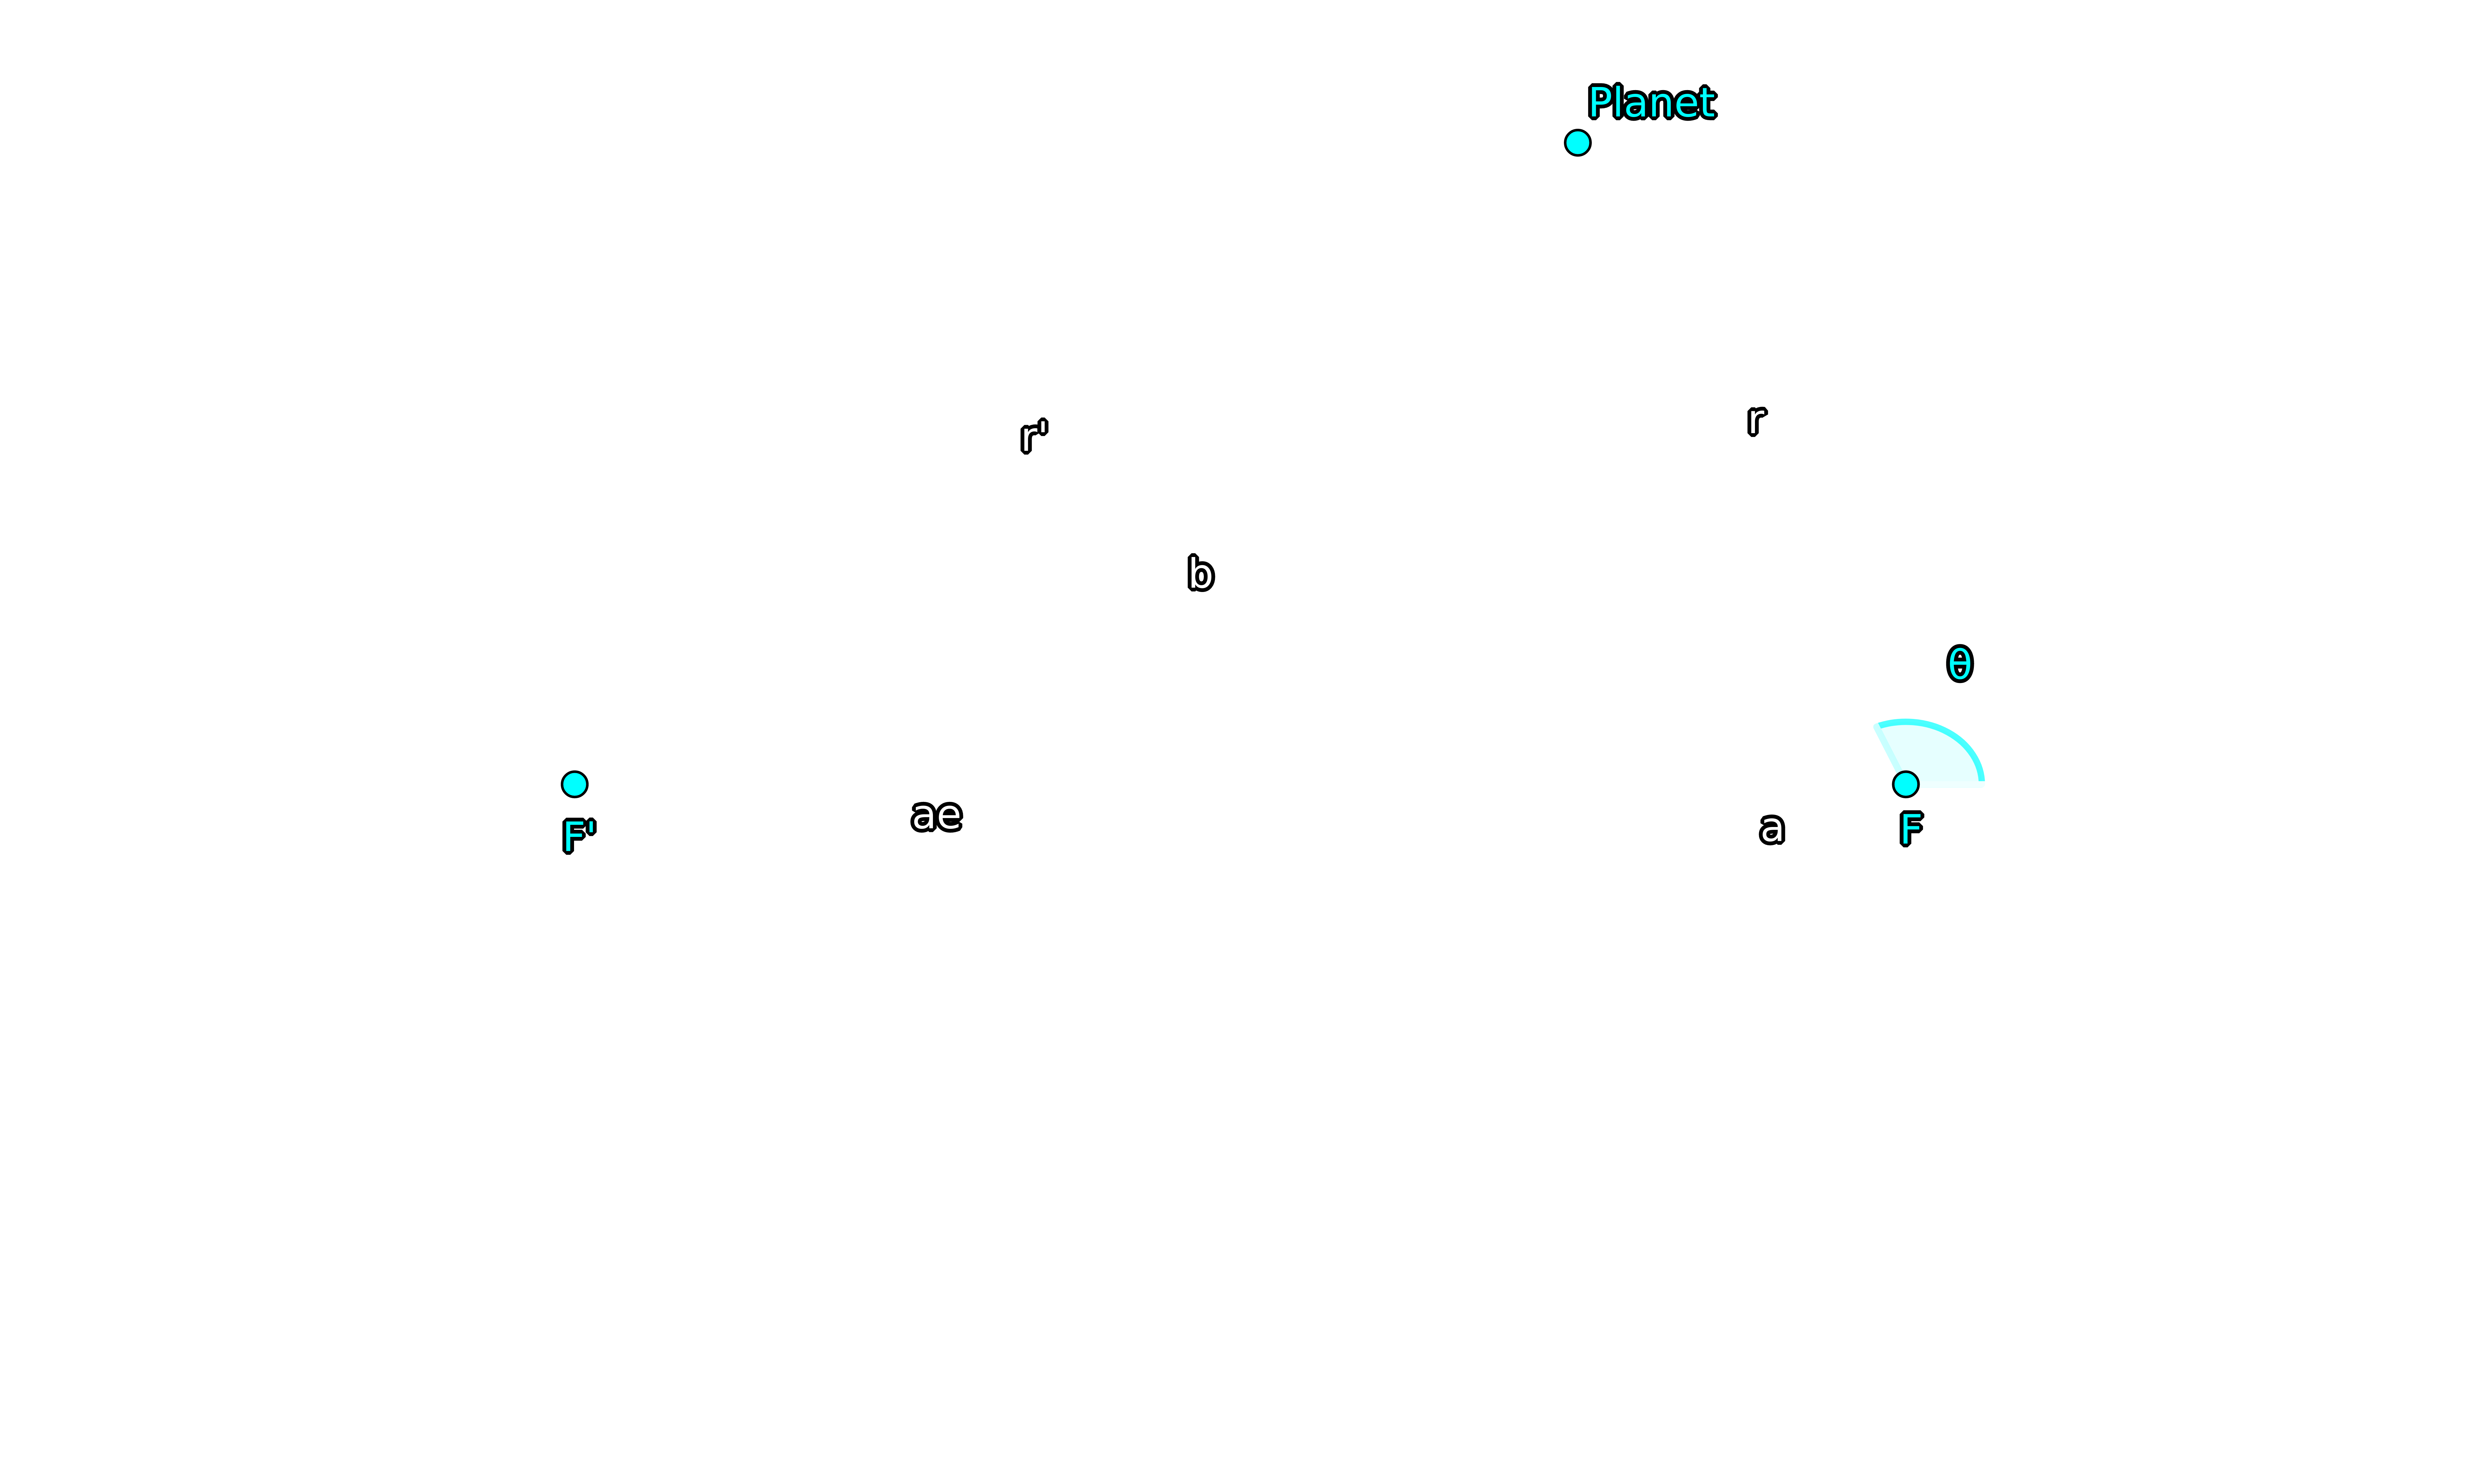
\includegraphics[width=\textwidth]{images/elliptical_orbit.png}
             \caption{Orbit of a planet}
             \label{fig:Orbit_ellpise}
         \end{figure}
     \end{frame}
    
    \begin{frame}{The Laws of Kepler Reloaded}
        \uncover<+->{\begin{equation}
        \label{ellipse_eqn}
            r = \frac{a(1-e^2)}{1 + e\cos \theta}
        \end{equation}}
        \uncover<+->{
        \begin{equation}
        \label{ang_mom_cons}
            r^2 \dv{\theta}{t} = {\rm constant}
        \end{equation}}
        \uncover<+->{
        \begin{equation*}
            P^2\ ({\rm in\ years}) = a^3\ ({\rm in\ AU})
        \end{equation*}}
    \end{frame}
    
    \begin{frame}{The Laws of Kepler Revolutions}
        \begin{equation}
            \vb{F} = -\frac{Gm_1m_2}{r^2}\vu{r}
            \label{NewtonsLaw}
        \end{equation}
        
    \end{frame}
	
	\subsection{Motivating Newton's Law}
	\frame{\sectionpage}
	\begin{frame}{Standing on the shoulders of giants (so not Hooke)}
		This is relatively simple to do with calculus
	\end{frame}
	
	\begin{frame}
	In plane polar co-ordinates, we have
	$$\vb{r}=r \hat{\vb{r}}$$
	$$\dot{\vb{r}}=\dot{r}\hat{\vb{r}}+r\dot{\theta}\hat{\bm{\theta}}$$
	$$\ddot{\vb{r}}=(\ddot{r}-r\dot{\theta}^2)\hat{\vb{r}}+(2\dot{r}\dot{\theta}+r\ddot{\theta})\hat{\bm{\theta}}$$
	That last term in the third equation looks familiar. 
	$ r^2 \dot{\theta} ={\rm constant }\implies 2r\dot{r}\dot{\theta} + r^2 \ddot{\theta} = 0$, so immediately, Kepler's second law implies that the gravitational force is radial (apart from the obvious(?) conservation law)
	
\end{frame}
	
	\begin{frame}
		Kepler's first law gives us
		$$r = \frac{a(1-e^2)}{1 + e\cos \theta}$$
		Differentiating with respect to time,
		$$\dot{r}=-\frac{l}{(1-e\cos{\theta})^2}e\sin{\theta}\;\dot{\theta}$$
		Now, we can use Kepler's second law ($\dot{A}=\frac{1}{2}r^2\dot{\theta}=k$) and substitute $\dot{\theta}$ in terms of $r$ and put back Kepler's first law to substitute for the $(1-e\cos{\theta})$ term in the denominator to eventually get
		$$\dot{r}=-\frac{2k}{l}e\sin{\theta}$$
		and differentiating again and simplifying as above, we get
		$$\ddot{r}=-\frac{4k}{l r^2}\left(1-\frac{l}{r} \right)$$
	\end{frame}
	
	\begin{frame}
		Now, we can write the acceleration $\ddot{\bm{r}}$ as
		$$\ddot{\bm{r}}=\left[-\frac{4k}{l r^2}\left(1-\frac{l}{r} \right)-r\left(\frac{2k}{l} \right)^2\right]\hat{\bm{r}} = -\frac{4k}{l r^2}\hat{\bm{r}}$$
		So, we get the force to be of the form, 
		$$\bm{F}=m\ddot{\bm{r}}=-\frac{4 m k/l}{r^2}\hat{\bm{r}}$$
	\end{frame}
	
	\begin{frame}{But wait...}
		\onslide*<1->{We have more: the planet's frame of motion. \\The same calculation will yield the same results, with the masses exchanged.}
		\\[3\baselineskip]
		\onslide+<2->{Confused?}
	\end{frame}
	\begin{frame}
		\begin{figure}
			\centering
			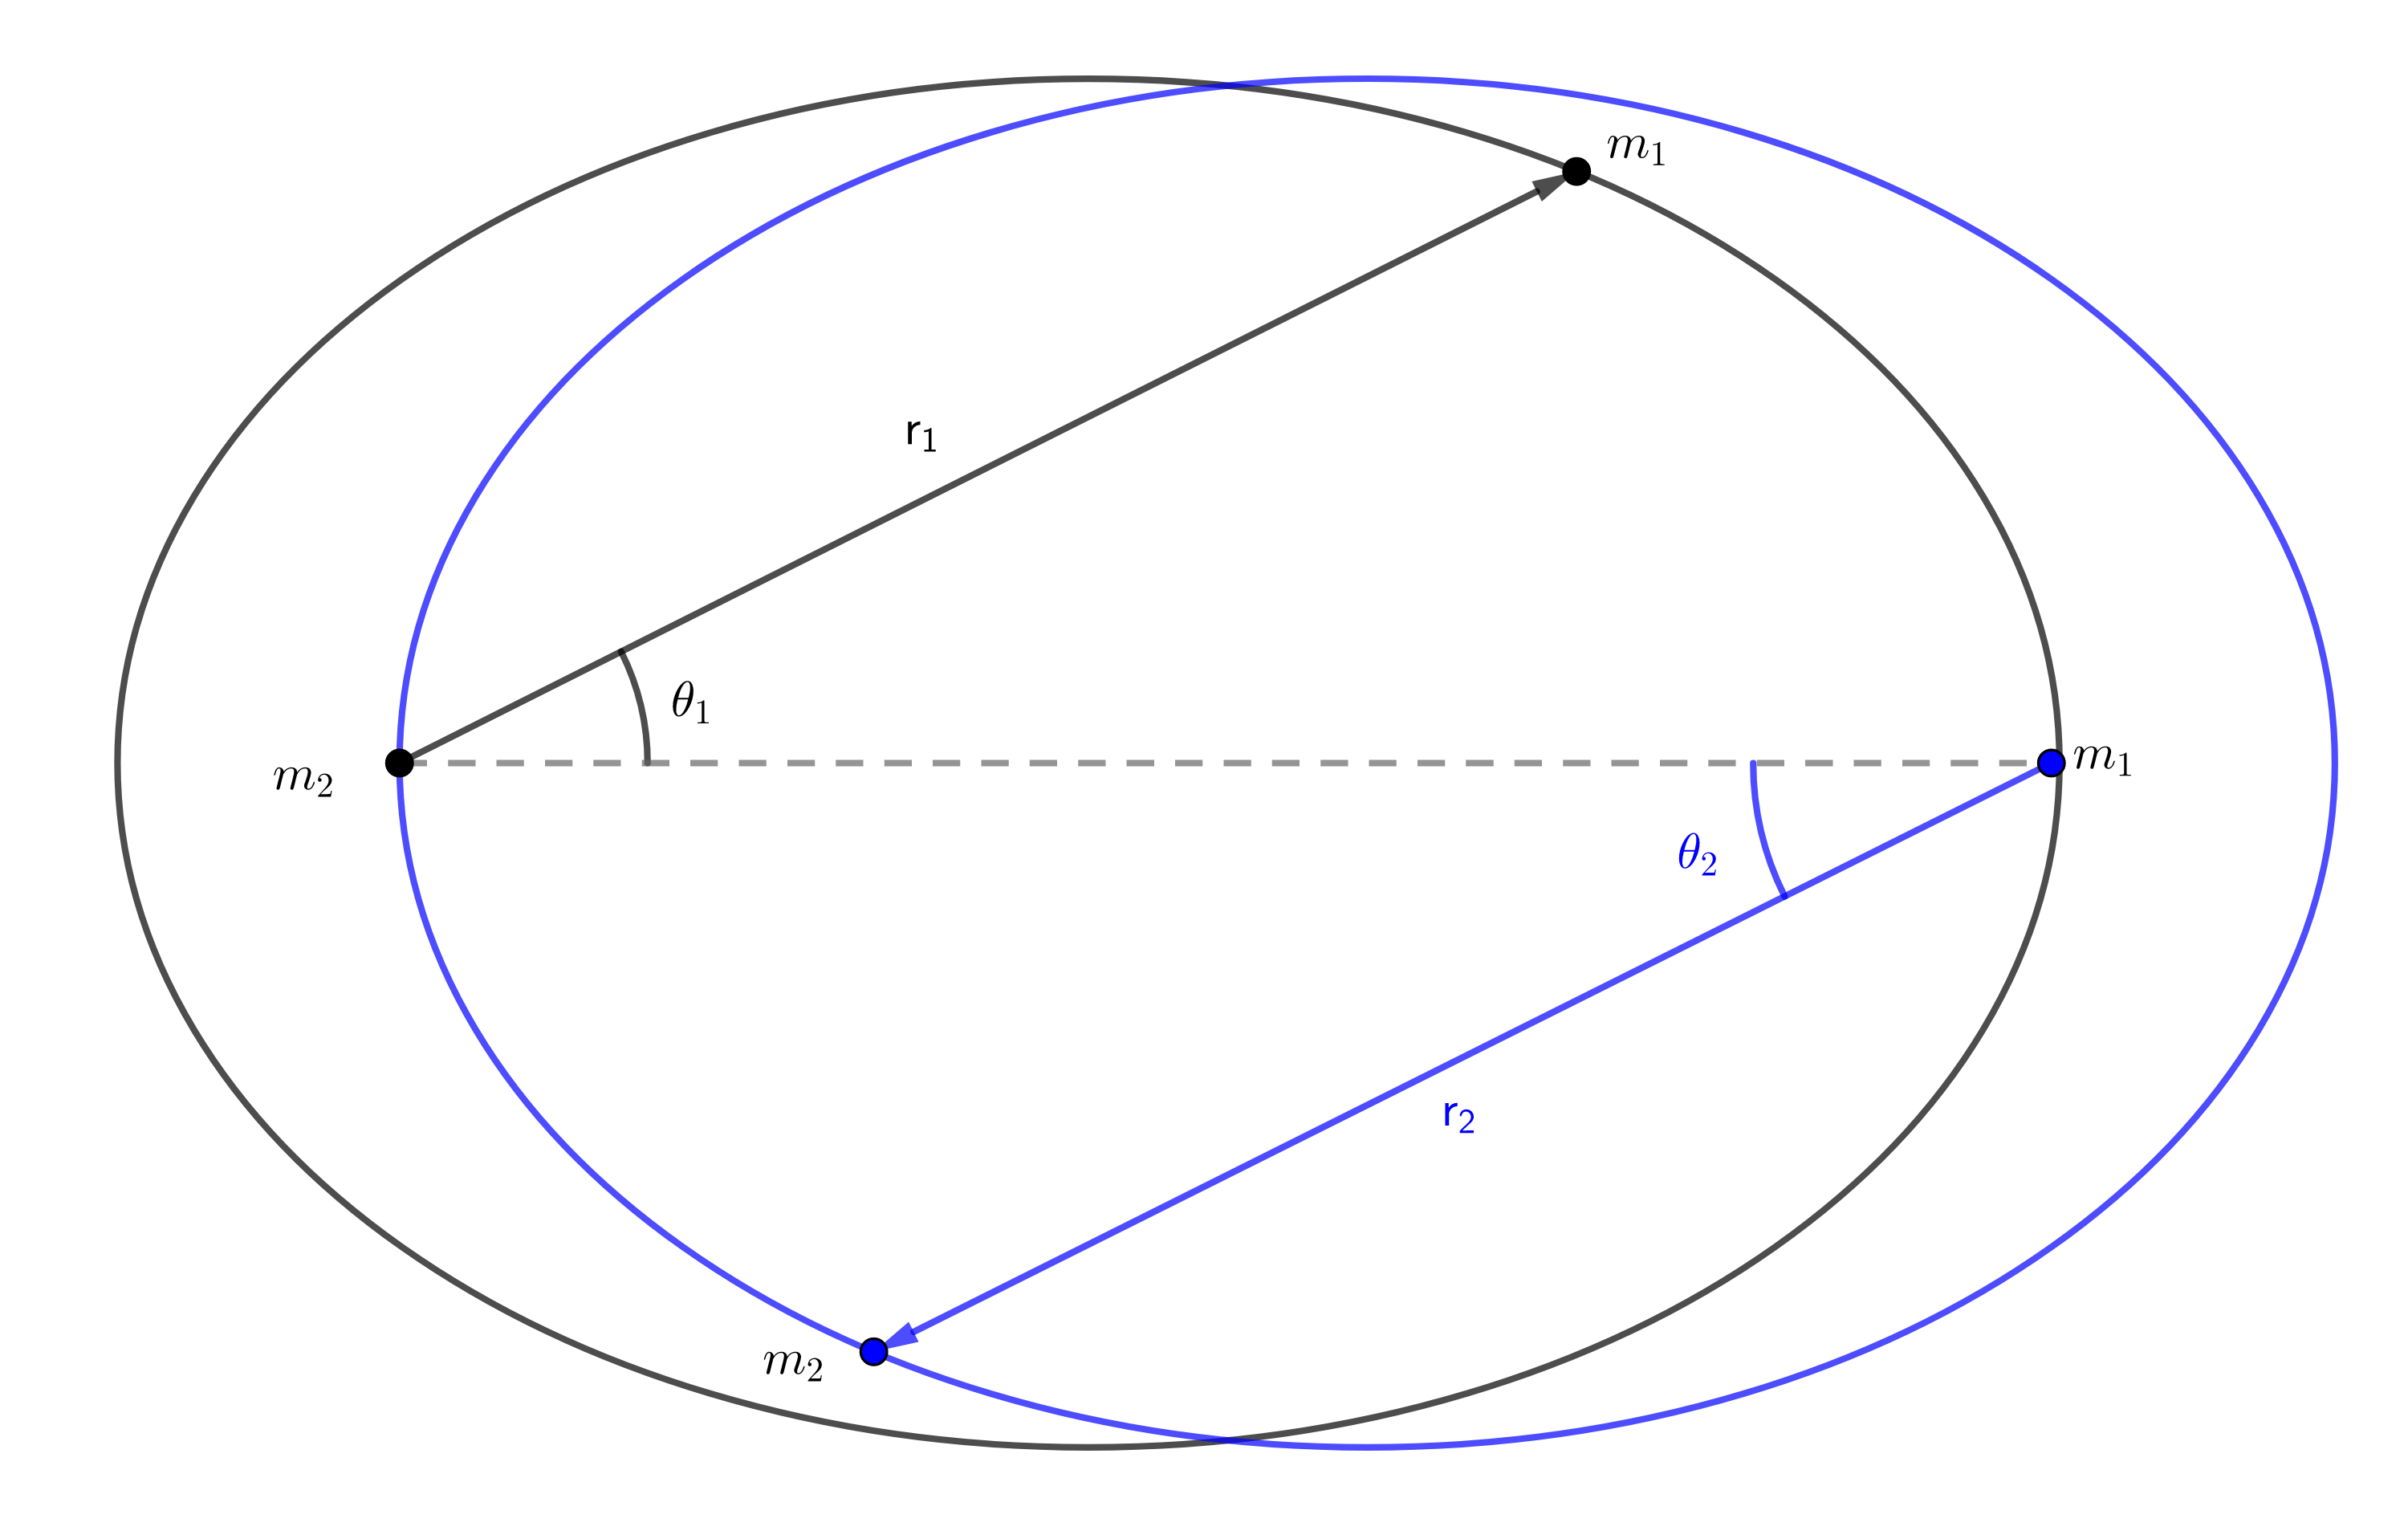
\includegraphics[width=\textwidth]{images/different_frames.png}
		\end{figure}
	\end{frame}

	\begin{frame}
		From the frame of $m_1$, we can write the force $\bm{F}_{12}$ exerted by $m_1$ on $m_2$ as
		$$\bm{F}_{12}=-\frac{4m_2 k_1}{l r_1^2}\hat{r_1}$$
		and conversely,
		$$\bm{F}_{21}=-\frac{4m_1 k_2}{l r_2^2}\hat{r_2}$$
		\newpage
		Now, using Newton's Third Law, and accounting for the fact that $r_1=r_2$ and $\hat{\bm{r}_1}=-\hat{\bm{r}_2}$, we get
		$$\bm{F}_{12}=-\bm{F}_{21}$$
		$$m_1 k_1=m_2 k_2$$
		i.e.
		$$\frac{k_1}{k_2}=\frac{m_2}{m_1}=\alpha$$
		$\alpha$ is a constant with respect to mass of the bodies, the distance between them and time. So, we can write the force as 
		$$\bm{F}_{12}=-\frac{4\alpha m_1 m_2}{r^2}\hat{\bm{r}}$$
	\end{frame}

	\begin{frame}
		This should make it obvious why Newton's Law looks the way that it does. 
		\begin{equation}
			\vb{F} = -\frac{Gm_1m_2}{r^2}\vu{r}
		\end{equation}
	\end{frame}
	
	
	
	 %You can put the frames directly into the presentation, but using the input command and writing them in separate .tex files might be more organized
    
     \section{apple}

\frame{\sectionpage}

\begin{frame}
	Now, we go the other way around. Let us assume Newton is right, and see what we get. \\
	From the fact that the force is central, we immediately get the Conservation of Angular Momentum, and are able to define a plane of motion of the two bodies.\\
\end{frame}

\begin{frame}
	The usual derivation is straightforward and lengthy (i.e. not fun), so we shall take the scenic route by considering the quantity (for any general central force, $\vb{F}=f(r)\hat{\vb{r}}$)
	\begin{align*}
		\dv{t}(\vb{p}\cross\vb{L}) &= \dot{\vb{p}}\cross \vb{L} = f(r) \hat{\bm{r}}\cross(m\vb{r}\cross \dot{\vb{r}})\\
		&= \frac{mf(r)}{r} \left (\vb{r}\cross(\vb{r}\cross\vb{\dot{r}})\right)\\
		&= \frac{mf(r)}{r} \left(r\dot{r} \vb{r} - r^2\vb{\dot{r}}\right)\\
		&= mf(r)r^2\left (\frac{\dot{r}\vb{r}}{r^2}-\frac{\vb{\dot{r}}}{r}\right )
	\end{align*}
	\begin{equation*}
		\dv{t}(\vb{p}\cross\vb{L}) = mf(r)r^2\dv{t}\left (\frac{\vb{r}}{r}\right )
	\end{equation*}
	If only $f(r)\ r^2$ were a constant of some sort. Then we could have a quantity called the Laplace-Runge-Lenz vector which would have been constant with time.
\end{frame}

\begin{frame}
	
	\onslide*<1->{We define
		\begin{equation*}
		\vb{A} = \vb{p}\cross\vb{L} - mk\hat{\vb{r}}
		\end{equation*}
		and we know that $\dot{\vb{A}} = 0$ from earlier (and $k=GMm$). 
		A very good question to ask at this point would be "What is this vector?" \\
		What is constant in the orbital motion of a planet?}
	\\[3\baselineskip]
	\onslide+<2->{The orbit.}	
\end{frame}

\begin{frame}
	\begin{figure}
		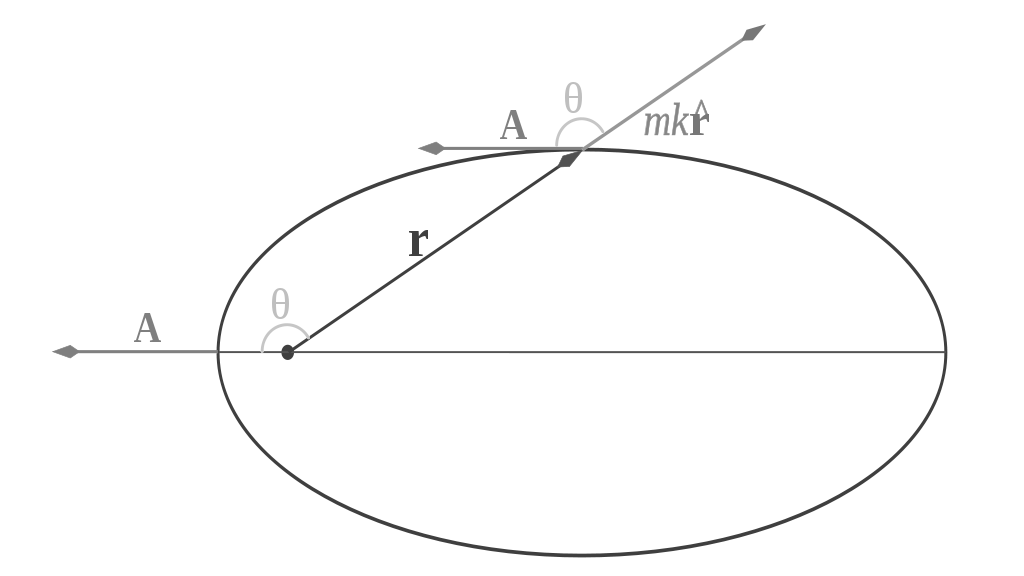
\includegraphics[width=\linewidth]{./images/LRL.png}
		\caption{\href{https://en.wikipedia.org/wiki/Laplace-Runge-Lenz\_vector}{Wikipedia}}
	\end{figure}
\end{frame}
\begin{frame}
	Since we want to know the variation of $\theta$ with $r$, we can take a dot product:
	\begin{equation*}
		\vb{A}\cdot\vb{r} = Ar \cos \theta = \vb{r}\cdot(\vb{p}\cross\vb{L}) - mkr
	\end{equation*}
	\begin{equation*}
		\vb{r}\cdot(\vb{p}\cross\vb{L})	= (\vb{r} \cross \vb{p})\cdot\vb{L} = \vb{L}\cdot\vb{L} = L^2
	\end{equation*}
	So, without any pain whatsoever, we have 
	\begin{equation*}
		r = \frac{L^2/mk}{1 + A/mk\cos\theta}
	\end{equation*}
	Note that $e = \frac{A}{mk}$, and so $\frac{\vb{A}}{mk}$ is often called the eccentricity vector.
\end{frame}

\begin{frame}
	Taking the dot product of $\vb{A}$ with itself gives the expression for energy in terms of the eccentricity
	\begin{equation*}
		A^2 = m^2k^2 + 2mEL^2
	\end{equation*}
	\begin{equation*}
		e^2 = 1 + \frac{2L^2}{mk^2}E
	\end{equation*}
	where $E = \frac{p^2}{2m} - \frac{k}{r}$
\end{frame}


    
    % \input{chapters/fourier-playground.tex}
    
%    \section*{Acknowledgments} %You can remove this if you do not want to use it
%        \begin{frame}{Acknowledgments}
%            The author is extremely thankful to Sir Isaac Newton, not just for the discoveries, but also for the sass. 
%        \end{frame}
    
    % \section*{References} %You can remove this if you do not want to use it
    %     \nocite{Djairo} \nocite{PhilPanof} \nocite{Fleming} \nocite{Shankar}
    %     \begin{frame}{References}
    %         \printbibliography
    %     \end{frame}

    \section{}
    \begin{frame}{}
        \centering
            \Huge\bfseries
        \textcolor{orange}{The End}
    \end{frame}
\end{document}
